\documentclass[10pt,twocolumn,letterpaper]{article}

\usepackage{cvpr}
\usepackage{times}
\usepackage{epsfig}
\usepackage{graphicx}
\usepackage{amsmath}
\usepackage{amssymb}

% Include other packages here, before hyperref.

% If you comment hyperref and then uncomment it, you should delete
% egpaper.aux before re-running latex.  (Or just hit 'q' on the first latex
% run, let it finish, and you should be clear).
\usepackage[pagebackref=true,breaklinks=true,letterpaper=true,colorlinks,bookmarks=false]{hyperref}

\usepackage{ifthen,color}
\definecolor{darkgreen}{rgb} {0.0,0.5,0.0}
\definecolor{darkblue}{rgb} {0.0,0.0,0.5}
\definecolor{bluegreen}{rgb}{0.0,0.5,0.5}
\newcommand{\todo}[1]           {{\color{red} #1}}
\newcommand{\yzh}[1]{{\it{\color{darkblue}(YZH) #1}}}
\newcommand{\yuduo}   [1]{{{\color{darkgreen}(John) #1}}}

\newcommand{\final}{0}
\ifthenelse{\equal{\final}{1}}{\renewcommand{\yuduo}[1]{}\renewcommand{\yzh}[1]{}}{}

\cvprfinalcopy % *** Uncomment this line for the final submission

\def\cvprPaperID{42} % *** Enter the CVPR Paper ID here
\def\httilde{\mbox{\tt\raisebox{-.5ex}{\symbol{126}}}}

% Pages are numbered in submission mode, and unnumbered in camera-ready
\ifcvprfinal\pagestyle{empty}\fi
\begin{document}

%%%%%%%%% TITLE
\title{Scene Classification with Deep Convolutional Neural Networks}

\author{Yangzihao Wang and Yuduo Wu\\
University of California, Davis\\
{\tt\small \{yzhwang,yudwu\}@ucdavis.edu}
% For a paper whose authors are all at the same institution,
% omit the following lines up until the closing ``}''.
% Additional authors and addresses can be added with ``\and'',
% just like the second author.
% To save space, use either the email address or home page, not both
}
\maketitle
%\thispagestyle{empty}

%%%%%%%%% ABSTRACT
\begin{abstract}
%summarize the problem, main idea, and results;
The use of massive datasets like ImageNet and the revival of Convolutional
Neural Networks (CNNs) for learning deep features has significantly improved
the performance of object recognition. However, performance at scene
classification has not achieved the same level of success since there is still
semantic gap between the deep features and the high-level context.  In this
project we proposed a novel scene classification method which combines CNN and
Spatial Pyramid to generate high-level context-aware features for one-vs-all
linear SVMs. Our method achieves the state-of-the-art result: 68.04\% average
accuracy rate on MIT indoor67 dataset using only the deep features trained from
ImageNet.

\end{abstract}

%%%%%%%%% BODY TEXT
\section{Related Work}
\label{sec:related}
%provide a detailed description of related papers (not necessarily limited to
%those in the schedule).  If you're proposing a new idea or extending an existing
%approach, compare and contrast it with existing work.  If you're analyzing one
%or two related techniques, describe how they relate to other relevant work;

Scene classification means to provide information about the semantic category or the function of a given image. Among different kidn of scene classification tasks, the indoor scene classification is considered to be one of the most difficult since the lack of discriminative features and contexts at the high level~\cite{Quattoni:2009:RIS}. Spatial pyramid representation\cite{Lazebnik:2006:BBF} is a popular method used for scene classification tasks. It is a simple and computationally efficient extension of an orderless bag-of-features image representation. However, without a proper high-level feature representation, such schemes often fail to offer sufficient semantic information of a scene. Object bank\cite{Li:2010:OBA} is among the first to propose a high-level image representation for scene classification. It uses a large number of pre-trained generic object detectors to create response maps for high level visual recognition tasks. The combination of off-the-shelf object detectors and a simple linear prediction model with a sparse-coding scheme achieves superior predictive power over similar linear prediction models trained on conventional representations. However, this method also limits the performance of their system to the performance of the object detectors they choose. Recently, Convolutional Neural Networks (CNNs) with flexible capacity makes training from large-scale dataset such as ImageNet~\cite{Deng:2009:IAL} possible. In the work of A. Krizhevsky et al.\cite{Krizhevsky:2012:ICD}, they trained one of the largest CNNs on the subsets of ImageNet and achieved better results than any other state-of-the-art methods in 2012. While their CNN system focuses on object detection, the features generated can be used for other applications such as scene classification. Two types of improvements has been done on top of their CNN works. The first type of improvement tries to address the problem of generating possible object locations in an image. Selective search method~\cite{Uijlings:2013:SSO} combines the strength of both an exhaustive search and segmentation and results in a small set of data-driven, class-independent, high quality locations. Girshick et al. propose the Regions with CNN features (R-CNN) method~\cite{Girshick:2013:RFH} as a more effective feature generation method. Alternatively, Zhou et al. try to increase the performance of scene classification using CNN by creating a new scene-centric database~\cite{Zhou:2014:LDF}.

%%%%%%%%% BODY TEXT
\section{Technical Approach}
\label{sec:method}
%Describe in detail the feature representation(s) and algorithm(s) you employed.
%The description should be self-contained (i.e., the reader should not have to
%rely on outside sources for your points to be clear), and should provide enough
%detail so that the reader could re-implement the approach.  Clearly state the
%method's input and output, and any assumptions or design choices;

\subsection{Selective Search}
Selective search is widely used for generating possible object locations for
use in object recognition\cite{Uijlings:2013:SSO}. Same strategies can be
adopted on indoor scene classification. For the indoor scenes that can be well
characterized by objects they contain, the selective search can exploit local
discriminative information with greatly reduced number of locations compared
to an exhaustive search.

\subsection{Feature Extraction}

\subsubsection{Max Pooling}

\subsection{Spatial Pyramid Matching}
For each image, a three-level spatial pyramid representation is used, resulting
$number images * number windows * (1 + 4 + 16)$ length feature vectors.

\section{Experiments}
\label{sec:results}
%Describe the experiments you conducted to evaluate the approach.  For each
%experiment, describe what you did, what was the main purpose of the experiment,
%and what you learned from the results. Provide figures, tables, and qualitative
%examples, as appropriate.

In this section, we evaluate our method on the MIT-indoor67 dataset. Suggested training and
testing list of images are used to do the training (80 images per class) and validation (20
images per class), all images are in jpeg format. We notice that several
pairs of categories are relatively easier to be confused and misclassified by the
SVMs with each other (For the detaled confusion matrix, please refer to Figure~\ref{fig:confusion_matrix} in the Appendix. Such examples include bakery and deli, living room and bedroom, as well as
bookstore and library. We show some sample training and testing images from these
pairs in Figure~\ref{fig:sample}. For the bakery and deli pair, they both contain very
similar patterns of breads and sandwiches on shelves. For the livingroom and bedroom
pair, some living room images may include bed or bed-like sofa, which is almost identical
to the beds and sofas in images from bedroom category. For the library and bookstore,
both contain identical shelves of books. It is very difficult, even for human beings, to distinguish
images between these two categories.

\begin{figure}[ht]
  \centering
  \includegraphics[width=0.45\textwidth]{img/dataset.pdf}
  \centering
  \caption{This figure contains some sample images from the MIT-indoor67 dataset.
For each row, left two columns are from the same category and right two columns are from
another. The first pair is bakery and deli, the second pair is living rooms and bedrooms, and the last pair is library and bookstore.}
\label{fig:sample}
\end{figure}

Multi-class classification is done with a 67 SVMs trained using one-versus-all rule, that is, each
classifier is learned to separate each class from the rest of classes. Test image is assigned the
label of the class with the highest confidence score. Scene classification performance is
evaluated by the average multi-class classification accuracy over all scene classes.

For comparison purpose, we implement with the same procedure but only use
the extracted layer 7 4096-dimensional feature vectors from Caffe. After we get
one feature vectors for each entire image, instead of perform spatial pyramid
and L2 normalization, we simply add labels and send them into the multi-class
SVMs. Validation image feature vectors are also generated in the same way.

% Table 1
\begin{table*}[ht]
        \caption{Comparison results on MIT-indoor67}
        \centering
        \begin{tabular}{l c c}
        \hline \hline
        Models                & Average Precision \\ \hline
        $l2$ Normlization + Selective Search + Spatial Pyramid & {\bf{68.2953\%}} \\
        Selective Search + Spatial Pyramid & 68.0469\% \\
        Entire Image CNN Features & 59.9507\% \\
        \hline
        \end{tabular}
        \label{tab:overall}
\end{table*}

\subsection{Quantitative Evaluation}
We compare our scene classification performance with two other methods: 1) using only the
features extracted from the entire image; 2) using selective search and spatial pyramid, but without the
$l2$ normalization. The summary of our performance comparison is listed in Table~\ref{tab:overall}.
Our method achieves a mean average precision (mAP) of 68.2953\% on dataset
MIT-indoor67. For comparison, we implement the same method using only 4096-dimensional
feature vectors extracted from Caffe without region proposals, spatial pyramid, and max-pooling.
Using selective search and spatial pyramid gives us a 8.1\% performance gain and introducing
the $l2$ normalization gives us an extra 0.25\% performance gain. In most categories, we perform much
better than the average precision. Some examples are shoes shop, bedroom, grocery store, hospital room and operating
room. We achieve 100\% precision on three categories: cloister, florist, and bowling. This is because the region proposals and spatial pyramid technique
allow us to better characterize the particular objects belong to the category. For those categories which achieve worst precision, the false positives are
not evenly distributed either, but are focused on some very sensible categories. For example the top two false positive categories for auditorium are concert hall
and movie theater.
We also note some drops of average accuracy using our methods. The drops mainly happen for on the following three categories: prison-cell, library and living room.
Note these three categories are all relatively easier to be characterized by global spatial properties (prison cell bars and books on shelves) so focusing on small regions
might suppress the representation of the global scene.

% top 5 best and top 5 worst table (Table 2)
\begin{table}[ht]
        \caption{Top 5 Best and Top 5 Worst Results}
        \centering
        \begin{tabular}{l l l}
        \hline \hline
        & Name           & Avg. Prec./Top FP Ctgr. \\ \hline
        \multirow{5}{*}{Top 5 Best}
        & cloister       & 100\% \\
        & florist        & 100\% \\
        & bowling        & 100\% \\
        & poolinside     & 95\% \\
        & greenhouse     & 94.74\% \\
        \hline
        \multirow{5}{*}{Top 5 Worst}
        & livingroom     & 20\%/bedroom \\
        & lobby          & 30\%/jelleryshop \\
        & deli           & 31.58\%/bakery \\
        & office         & 33.33\%/computer\_room \\
        & airport inside & 35\%/subway \\
        \hline
        \end{tabular}
        \label{tab:overall}
\end{table}

Table~\ref{tab:compare} compares the performance of our method against various other scene classification methods. Note that methods using CNNs all show significant improvements of the performance.
Also, our method which uses selective search and spatial pyramid achieves better performance than Zhou et al.'s work on both ImageNet-CNN and Places-CNN, a CNN trained on a dataset specific created for places.

% compare with other paper results
% Table 3
\begin{table}[ht]
        \caption{Comparison to other methods}
        \centering
        \begin{tabular}{l c c}
        \hline \hline
        Method                & Average Precision \\ \hline
        Object Bank~\protect\cite{Li:2010:OBA} & 37.6 \\
        DPM+GIST-color+SP~\protect\cite{Pandey:2011:SRW} & 43.1 \\
        ImageNet-CNN feature~\protect\cite{Zhou:2014:LDF} & 56.79 \\
        Places-CNN feature~\protect\cite{Zhou:2014:LDF} & 68.24 \\
        Our Method & 68.3 \\
        \hline
        \end{tabular}
        \label{tab:compare}
\end{table}

% heatmap visulizations
\subsection{Qualitative Evaluation}
\begin{figure}[ht]
  \centering
  \includegraphics[width=0.45\textwidth]{img/tp.pdf}
  \centering
  \caption{True Positive Test examples. An example consists of the original test image (left) and the heatmap represented the highest response regions during the prediction (right). First row: bedroom (left) and deli (right); second row: livingroom (left) and lobby (right); and third row: airport\_inside (left) and office (right).}
  \label{fig:tp}
\end{figure}

For qualitative evaluation, we show samples of the true positive test examples in Figure~\ref{fig:tp}. Note that the selective search and spatial pryamid enable the algorithm to use the most informative region as the highest response during the prediction process. For example, in the bedroom example, highest responses are from bed and pollows; in the livingroom example, highest responses are from sofa and coffe table; and in the office example, desk and cabinet shelf. In large scenes, the highest responses are also focused around characteristic regions (airport\_inside's feature region is the glass ceiling and  the lobby's feature region is the checkin desk).

% heatmap visulizations
\begin{figure}[ht]
  \centering
  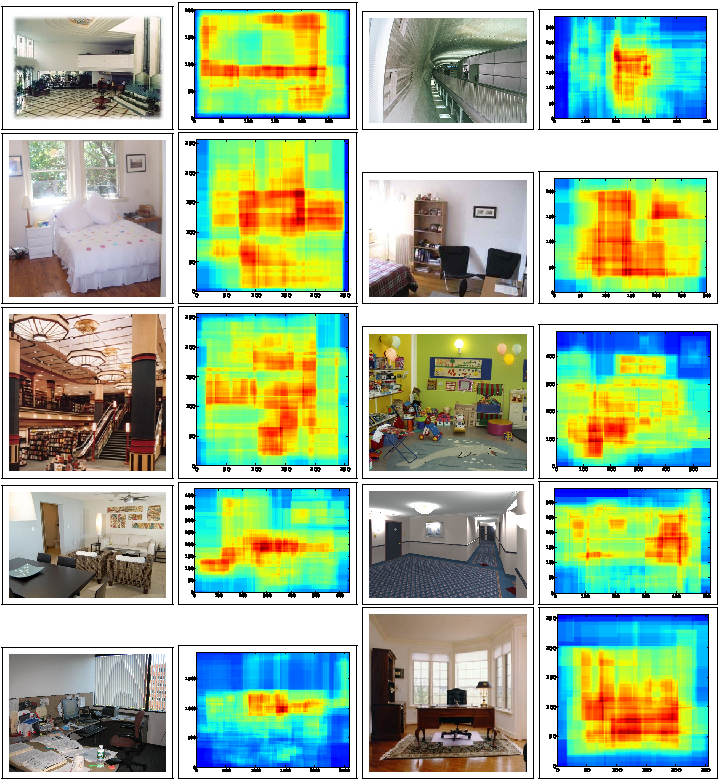
\includegraphics[width=0.45\textwidth]{img/fp.pdf}
  \centering
  \caption{False Positive Test examples. An example consists of the original test image (left) and the heatmap represented the highest response regions during the prediction (right). First row: lobby/airport\_inside (left) and subway/airport\_inside (right); second row: nursery/bedroom (left) and waitingroom/bedroom (right); third row: staircase/airport\_inside (left) and kindergarden/children\_room (right); forth row: bathroom/livingroom (left) and lockerroom/lobby (right); and fifth row: computerroom/office (left) and livingroom/office (right).}
  \label{fig:tp}
\end{figure}

The false positive test examples show some misclassification examples. The reasons are as follows: 1) Overfitting to the training sets. For example, airport inside which looks like a lobby or a subway station,  bedroom which looks like a nursery room, lobby which contains staircase in the scene, children room which contains too many toys that might appear more often in kindergarden category in the training set. 2) Wrong recognitions of key objects. For example in the bathroom/livingroom example recognizing the plate on the table as a hand washing sink, and in the lockerroom/lobby example recognizing the room doors as safe cases. 3) Failing the consider key objects. For example, in the waitingroom/bedroom example, the bed in the lower left corner is ignored by responses, and in the computerroom/office example, the desktop full of books and documents are also ignored. The false positive test examples show two places where we can improve the current model: First, a better method for extract regions of interest can be applied to increase the performance of selective search. Second, by carefully design better training dataset, the false positive cases will also be reduced.







%-------------------------------------------------------------------------
\section{Conclusions}

briefly summarize the main idea and results, and possible future work.

{\small
\bibliographystyle{ieee}
\bibliography{report}
}

\appendix
\section*{Appendix: Confusion Matrix}

\label{sec:appendix}
% confusion matrix
\FloatBarrier
\begin{figure}[h!]
  \centering
  \includegraphics[width=0.95\textwidth]{img/matrix.pdf}
  \centering
  \caption{Confusion matrix of prediction results for 67 categories.}
  \label{fig:confusion_matrix}
\end{figure}
\FloatBarrier

\end{document}